\documentclass[aspectratio=169]{beamer}

\usepackage[utf8]{inputenc}
\usepackage[english]{babel}
\usepackage{graphicx}
\usepackage{booktabs}
\usepackage{amsmath}
\usepackage{xcolor}

% ============================================================
%  HUST brand palette — chỉnh 1 dòng dưới đây nếu cần đổi đỏ
% ============================================================
\definecolor{hustred}{HTML}{C8102E}    % <-- màu chủ đạo (HUST red)
\definecolor{hustdark}{HTML}{8E0B20}   % sắc đậm hơn: nhấn / alert
\definecolor{husttint}{HTML}{FBEEF0}   % nền nhạt cho block
\definecolor{hustgray}{HTML}{404040}

\usetheme{Madrid}
\usecolortheme{default}

% --- áp màu vào toàn bộ theme ---
\setbeamercolor{structure}{fg=hustred}
\setbeamercolor{palette primary}{bg=hustred,  fg=white}
\setbeamercolor{palette secondary}{bg=hustdark, fg=white}
\setbeamercolor{palette tertiary}{bg=hustdark, fg=white}
\setbeamercolor{titlelike}{parent=structure}
\setbeamercolor{title}{bg=hustred, fg=white}
\setbeamercolor{subtitle}{fg=white}
\setbeamercolor{frametitle}{bg=hustred, fg=white}
\setbeamercolor{author}{fg=hustgray}
\setbeamercolor{institute}{fg=hustgray}

\setbeamercolor{block title}{bg=hustred, fg=white}
\setbeamercolor{block body}{bg=husttint, fg=black}
\setbeamercolor{block title alerted}{bg=hustdark, fg=white}
\setbeamercolor{block body alerted}{bg=husttint, fg=black}
\setbeamercolor{alerted text}{fg=hustdark}

\setbeamercolor{itemize item}{fg=hustred}
\setbeamercolor{itemize subitem}{fg=hustred}
\setbeamercolor{enumerate item}{fg=hustred}
\setbeamercolor{caption name}{fg=hustred}

\setbeamertemplate{navigation symbols}{}
\setbeamertemplate{caption}[numbered]
\setbeamerfont{frametitle}{series=\bfseries}
\setbeamerfont{footnote}{size=\tiny}

\graphicspath{{../report/figures/}}

% Custom colours for emphasis (xanh dương đậm tương phản tốt với nền đỏ)
\definecolor{good}{RGB}{0,105,80}
\newcommand{\good}[1]{\textcolor{good}{\textbf{#1}}}
\newcommand{\warn}[1]{\textcolor{hustdark}{\textbf{#1}}}

\title[Fraud Detection]{Real-Time Payment Fraud Detection}
\subtitle{Business Analytics Group Project --- Modules 1--8}
\author[Team]{[Team member names]}
\institute[]{Business Analytics}
\date{}

\begin{document}

% ---------------- 1
\begin{frame}
\titlepage
\end{frame}

% ---------------- 2
\begin{frame}{Agenda}
\begin{columns}[T]
\begin{column}{0.5\textwidth}
\begin{enumerate}
    \item Business problem \& KPIs \hfill \textit{(M1)}
    \item Two data sources \hfill \textit{(M1)}
    \item \warn{The leakage trap} \hfill \textit{(design)}
    \item Key EDA findings \hfill \textit{(M2)}
    \item Data cleaning decisions \hfill \textit{(M3)}
\end{enumerate}
\end{column}
\begin{column}{0.5\textwidth}
\begin{enumerate}
    \setcounter{enumi}{5}
    \item Feature engineering \hfill \textit{(M4)}
    \item Model results \& cost threshold \hfill \textit{(M5)}
    \item \warn{What our numbers really mean}
    \item Deploy: API $+$ review queue \hfill \textit{(M6)}
    \item Monitoring $+$ retraining \hfill \textit{(M7)}
    \item Risk policy \hfill \textit{(M8)} $+$ conclusion
\end{enumerate}
\end{column}
\end{columns}

\vspace{1em}
\begin{block}{The one thing to remember}
Our best model reaches PR-AUC $0.997$ --- and the interesting part is
\warn{why that number is not as impressive as it looks}.
\end{block}
\end{frame}

% ---------------- 3
\begin{frame}{1. The business problem}
\begin{block}{The question we must answer}
\emph{``Which transactions are likely fraudulent, and how should the platform
balance blocking fraud against approving legitimate orders without
unnecessary friction?''}
\end{block}

\vspace{0.5em}
\begin{columns}[T]
\begin{column}{0.5\textwidth}
\textbf{Fraud is costly}
\begin{itemize}
    \item Only \good{0.129\%} of transactions
    \item But \good{$8.2\times$ larger} on average
    \item Total exposure: \good{$\approx 12.1$ billion}
\end{itemize}
\end{column}
\begin{column}{0.5\textwidth}
\textbf{But blocking is costly too}
\begin{itemize}
    \item Every false alarm $=$ a rejected customer
    \item Friction $\to$ abandoned carts, churn
    \item Goal is \emph{not} ``catch everything''
\end{itemize}
\end{column}
\end{columns}

\vspace{0.8em}
\centering
\alert{$\Rightarrow$ Find the operating point that minimizes \textbf{total business cost}}
\end{frame}

% ---------------- 4
\begin{frame}{1. KPIs we track}
\begin{table}
\centering
\begin{tabular}{lll}
\toprule
KPI & What it measures & Baseline \\
\midrule
Fraud rate & Risk exposure \& imbalance & $0.129\%$ \\
False-positive rate & Customer friction & to minimize \\
Financial loss avoided & Business value & target \\
\bottomrule
\end{tabular}
\end{table}

\vspace{1em}
\begin{alertblock}{Why accuracy is useless here}
A model that predicts ``never fraud'' achieves \textbf{99.87\% accuracy}
and catches \textbf{zero} fraud.\\
$\Rightarrow$ We use \good{PR-AUC}, Recall, $F_1$ --- never accuracy.
\end{alertblock}
\end{frame}

% ---------------- 5
\begin{frame}{2. Two data sources}
\begin{columns}[T]
\begin{column}{0.5\textwidth}
\textbf{Source 1 --- PaySim (Kaggle)}
\begin{itemize}
    \item $6{,}362{,}620$ transactions
    \item 743 hourly steps ($\approx$ 31 days)
    \item Balances before/after, type, amount
    \item Ground-truth \texttt{isFraud}
\end{itemize}
\end{column}
\begin{column}{0.5\textwidth}
\textbf{Source 2 --- Synthetic (Faker)}
\begin{itemize}
    \item \textbf{10 contextual features}
    \item Account age, home country, device
    \item New-device flag, address mismatch
    \item Failed attempts, IP distance
    \item Fully documented in a data dictionary
\end{itemize}
\end{column}
\end{columns}

\vspace{1em}
\begin{block}{Generation was label-conditional --- on purpose}
e.g.\ \texttt{is\_new\_device}: $p = 0.55$ if fraud, $0.08$ if legitimate\\
\texttt{failed\_payment\_attempts}: Poisson $\lambda = 2.2$ vs $0.12$
\end{block}
\end{frame}

% ---------------- 5b (data dictionary)
\begin{frame}{2. Documenting every synthetic field}
The brief requires a \textbf{data dictionary}: each generated field must state
its name, type, unit, valid range, and generation logic.

\begin{table}
\centering
\scriptsize
\begin{tabular}{lll}
\toprule
Field (type $\cdot$ unit) & Range & Generation logic (fraud vs.\ legit) \\
\midrule
\texttt{account\_age\_days} (int $\cdot$ day)   & 1--3650       & Gamma; mean $\approx 44$ vs $500$ \\
\texttt{is\_new\_device} (0/1)                   & \{0,1\}       & Bernoulli $p = 0.55$ vs $0.08$ \\
\texttt{ip\_billing\_mismatch} (0/1)             & \{0,1\}       & Bernoulli $p = 0.50$ vs $0.02$ \\
\texttt{failed\_payment\_attempts} (int)         & $0$--$\sim$10 & Poisson $\lambda = 2.2$ vs $0.12$ \\
\texttt{ip\_billing\_distance\_km} (km)          & 0--8000       & Uniform$(500,8000)$ if mismatch, else $(0,80)$ \\
\bottomrule
\end{tabular}
\end{table}

\begin{columns}[T]
\begin{column}{0.5\textwidth}
\good{10 contextual fields} documented in total\\
(\texttt{channel} is EDA-only; 7 risk signals feed the model)
\end{column}
\begin{column}{0.5\textwidth}
Exported as \texttt{data\_dictionary.\{md,csv,xlsx\}}\\
\footnotesize Reproducible from a single notebook cell.
\end{column}
\end{columns}

\vspace{0.4em}
\centering
\footnotesize The label-conditional parameters above are exactly what makes the
\warn{leakage} measurable (next slides).
\end{frame}

% ---------------- 6
\begin{frame}{3. The trap we found in our own data}
Our synthetic features separate the classes beautifully:

\begin{table}
\centering
\small
\begin{tabular}{lrrr}
\toprule
Feature & Legitimate & Fraud & Ratio \\
\midrule
\texttt{account\_age\_days}        & 500.1 & 44.1   & $0.09\times$ \\
\texttt{is\_new\_device}           & 0.080 & 0.551  & $6.9\times$ \\
\texttt{failed\_payment\_attempts} & 0.120 & 2.249  & $18.7\times$ \\
\texttt{ip\_billing\_mismatch}     & 0.020 & 0.499  & $25.0\times$ \\
\bottomrule
\end{tabular}
\end{table}

\begin{alertblock}{But we generated them \emph{from} the label}
Their predictive power is \warn{by design}, not discovered.
Using them naively would be \warn{label leakage} --- we would be grading
our own homework.
\end{alertblock}

\centering
\alert{Our solution: build \textbf{two} feature spaces and compare them everywhere.}
\end{frame}

% ---------------- 7
\begin{frame}{3. The Base / Full design}
\begin{columns}[T]
\begin{column}{0.48\textwidth}
\begin{block}{Base --- 11 features (no leakage)}
Real PaySim data only
\begin{itemize}
    \item amount, 4 balance columns
    \item \texttt{errorBalance*} (engineered)
    \item \texttt{type\_TRANSFER}
    \item velocity, time-since-last
\end{itemize}
\good{No leakage} --- honest difficulty
\end{block}
\end{column}
\begin{column}{0.48\textwidth}
\begin{block}{Full --- 18 features (leaky)}
Base $+$ 7 synthetic risk signals
\begin{itemize}
    \item account age, device flag
    \item address / IP mismatch
    \item failed attempts, IP distance
\end{itemize}
\warn{Leaky} --- optimistic upper bound
\end{block}
\end{column}
\end{columns}

\vspace{1em}
\centering
Every algorithm is trained on \textbf{both}.\\
\alert{The gap between them \emph{measures} the leakage instead of hiding it.}
\end{frame}

% ---------------- 8
\begin{frame}{4. EDA: two findings that shaped everything}
\begin{columns}[T]
\begin{column}{0.5\textwidth}
\textbf{(a) Fraud lives in only 2 of 5 types}
\begin{table}
\scriptsize
\begin{tabular}{lrr}
\toprule
Type & Fraud & Rate \\
\midrule
CASH\_OUT & 4{,}116 & 0.184\% \\
TRANSFER  & 4{,}097 & \good{0.769\%} \\
CASH\_IN  & 0 & 0\% \\
PAYMENT   & 0 & 0\% \\
DEBIT     & 0 & 0\% \\
\bottomrule
\end{tabular}
\end{table}
$\Rightarrow$ Filter to 2 types: positive rate\\
\good{$0.129\% \to 0.296\%$} at zero information cost
\end{column}
\begin{column}{0.5\textwidth}
\textbf{(b) Fraud breaks the accounting identity}
\begin{align*}
\texttt{errBalOrig} &= \texttt{newBal} + \texttt{amt} - \texttt{oldBal}
\end{align*}
Fraud \emph{drains} the origin account, leaving an arithmetic footprint.

\vspace{0.5em}
Naive rule ``account emptied'':\\
fraud rate only $0.223\%$ ($1.7\times$)

\vspace{0.3em}
\alert{The \emph{error} formulation is far sharper}\\
$\to$ becomes our top feature
\end{column}
\end{columns}
\end{frame}

% ---------------- 8b (EDA by channel)
\begin{frame}{4. EDA: fraud rate by transaction channel}
\begin{center}
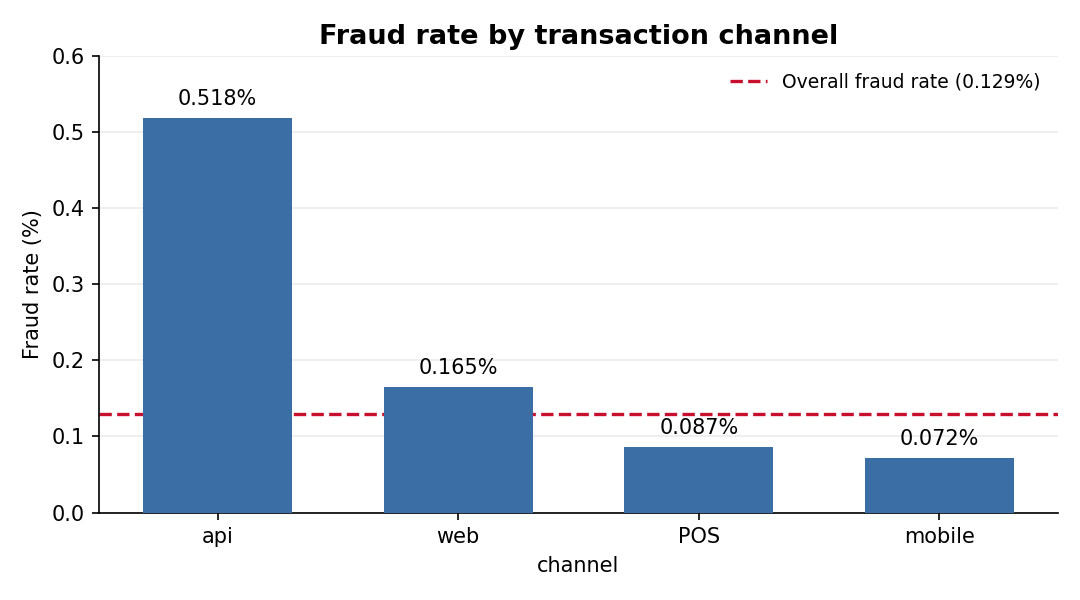
\includegraphics[height=0.52\textheight]{fraud_rate_channel.png}
\end{center}

\begin{columns}[T]
\begin{column}{0.56\textwidth}
\texttt{api} and \texttt{web} sit \good{above} the $0.129\%$ average;
\texttt{POS} and \texttt{mobile} below it.
\texttt{api} runs \good{$\approx 7\times$} the \texttt{mobile} rate.
\end{column}
\begin{column}{0.44\textwidth}
\footnotesize
\texttt{channel} is a \emph{synthetic, EDA-only} field, so this split partly
reflects how it was generated --- reported as description, not proof.
\end{column}
\end{columns}

\vspace{0.3em}
\centering
\footnotesize Fraud rate by hour-of-day (\texttt{step} mod $24$) was also examined in the notebook.
\end{frame}

% ---------------- 9
\begin{frame}{5. Cleaning: the decision we are proudest of}
\begin{columns}[T]
\begin{column}{0.52\textwidth}
\textbf{What we found}
\begin{itemize}
    \item 0 missing values, 0 duplicates
    \item 16 invalid rows removed
    \item IQR rule flags \textbf{338{,}077} outliers (5.31\%)
\end{itemize}

\vspace{0.6em}
\textbf{The textbook says: remove outliers}
\end{column}
\begin{column}{0.44\textwidth}
\begin{alertblock}{We kept them --- here is why}
Fraud rate \emph{inside} the outlier group:\\
\centering \good{1.14\%} vs $0.129\%$ overall\\
$= 8.8\times$ denser in fraud
\end{alertblock}
\end{column}
\end{columns}

\vspace{0.8em}
\centering
\alert{Clipping the tail would have deleted our rare positives.}\\
In fraud detection, a large amount is \textbf{signal}, not noise.

\vspace{0.6em}
\footnotesize
Every cleaning step logged rows \emph{and} fraud removed --- verified with assertions.
\end{frame}

% ---------------- 10
\begin{frame}{6. Feature engineering \& imbalance}
\begin{columns}[T]
\begin{column}{0.5\textwidth}
\textbf{Handling $1{:}337$ imbalance}
\begin{itemize}
    \item Class weights in \emph{all} 3 models
    \item LogReg: \texttt{balanced}
    \item XGBoost: \texttt{scale\_pos\_weight} $\approx 337$
    \item RF: \texttt{balanced\_subsample}
\end{itemize}
\footnotesize All impose the \emph{same} $337{:}1$ penalty $\Rightarrow$ fair comparison.
\end{column}
\begin{column}{0.5\textwidth}
\textbf{Feature selection (mutual information)}
\begin{itemize}
    \item MI ranks \texttt{errorBalanceOrig} only 5th\ldots
    \item \ldots yet it is the \#1 feature in the models
    \item MI is \emph{univariate}, blind to interactions
\end{itemize}
\alert{$\Rightarrow$ We kept all features.}\\
\footnotesize Blind pruning would have deleted our best predictor.
\end{column}
\end{columns}

\vspace{0.8em}
\begin{block}{An honest negative result}
Required velocity features (\texttt{txn\_count\_acct},
\texttt{time\_since\_last\_txn}) are \textbf{degenerate on PaySim} ---
accounts almost never repeat (mean count $= 1.00$).
Built correctly, but carry \textbf{zero} importance.
\end{block}
\end{frame}

% ---------------- 11
\begin{frame}{7. Results: 3 algorithms $\times$ 2 feature spaces}
\begin{table}
\centering
\small
\begin{tabular}{lccccc}
\toprule
Model & PR-AUC & Recall & Precision & FP & FN \\
\midrule
LogReg $\cdot$ Base       & 0.5932 & 0.9081 & 0.0433 & \warn{49{,}287} & 226 \\
LogReg $\cdot$ Full       & 0.9704 & 0.9947 & 0.3348 & 4{,}860 & 13 \\
\textbf{RF $\cdot$ Base}  & \good{0.9976} & 0.9967 & 0.9996 & \good{1} & 8 \\
RF $\cdot$ Full           & 0.9997 & 0.9963 & 1.0000 & 0 & 9 \\
XGBoost $\cdot$ Base      & 0.9944 & 0.9931 & 0.9222 & 206 & 17 \\
XGBoost $\cdot$ Full      & 0.9996 & 0.9984 & 0.9923 & 19 & 4 \\
\bottomrule
\end{tabular}
\end{table}

\begin{columns}[T]
\begin{column}{0.5\textwidth}
\alert{Random Forest Base} --- best \emph{honest} model:\\
\good{1 false positive} out of $828{,}659$\\
using \textbf{no synthetic data at all}
\end{column}
\begin{column}{0.5\textwidth}
\warn{LogReg Base} is unusable:\\
$22$ false alarms per fraud caught\\
\footnotesize (a hyperplane cannot express the balance interaction)
\end{column}
\end{columns}
\end{frame}

% ---------------- 12
\begin{frame}{7. Precision--Recall curves}
\begin{center}
\includegraphics[height=0.72\textheight]{pr_curves.png}
\end{center}
\centering
\footnotesize
The linear baseline degrades steadily; the four tree curves hug the corner.
\end{frame}

% ---------------- 13
\begin{frame}{8. Measuring the leakage we warned about}
\begin{table}
\centering
\begin{tabular}{lccc}
\toprule
Algorithm & Base & Full & Uplift from synthetic data \\
\midrule
Logistic Regression & 0.5932 & 0.9704 & \warn{$+0.3772$} \\
Random Forest       & 0.9976 & 0.9997 & \good{$+0.0021$} \\
XGBoost             & 0.9944 & 0.9996 & \good{$+0.0052$} \\
\bottomrule
\end{tabular}
\end{table}

\vspace{0.8em}
\begin{block}{What this tells us}
\begin{itemize}
    \item The leakage is \warn{real} --- it lifts the weak model by $+0.38$
    \item But it is \good{not load-bearing} --- tree models gain almost nothing
    \item Our best honest model (RF Base) \good{needs none of it}
\end{itemize}
\end{block}

\centering
\alert{Conclusion: our headline result does not rest on leaked information.}
\end{frame}

% ---------------- 14
\begin{frame}{8. Where the signal actually comes from}
\begin{columns}[c]
\begin{column}{0.62\textwidth}
\includegraphics[width=\textwidth]{feature_importance.png}
\end{column}
\begin{column}{0.36\textwidth}
\textbf{\good{Teal}} $=$ real PaySim\\
\textbf{\warn{Orange}} $=$ synthetic

\vspace{1em}
\begin{itemize}
    \item \texttt{errorBalanceOrig} alone $= \good{53.7\%}$
    \item Synthetic total $\approx 28\%$
    \item Velocity features $= \warn{0.000}$
\end{itemize}

\vspace{0.8em}
\alert{The tallest bar is a \emph{real} feature.}
\end{column}
\end{columns}
\end{frame}

% ---------------- 15
\begin{frame}{9. From probability to a business decision}
The default threshold $0.5$ has \emph{no business meaning}. We convert the
trade-off into money:

\begin{equation*}
\mathrm{Cost}(t) = \underbrace{\sum_{\text{missed fraud}} \texttt{amount}_i}_{\text{money lost}}
\;+\; \underbrace{C_{FP} \times \#\text{false alarms}}_{\text{friction, } C_{FP}=10}
\end{equation*}

\begin{center}
\includegraphics[height=0.45\textheight]{cost_threshold.png}
\end{center}

\centering
\alert{Optimal $t^{*} = 0.17$, not $0.5$ $\Rightarrow$ total cost $-14.7\%$}
\end{frame}

% ---------------- 16
\begin{frame}{9. The business outcome}
\begin{table}
\centering
\begin{tabular}{lr}
\toprule
Indicator (test set) & Value \\
\midrule
Fraud value at risk        & $3{,}615{,}247{,}576$ \\
\good{Fraud value stopped} & \good{$3{,}613{,}891{,}825$ \;($99.96\%$)} \\
Fraud value leaked         & $1{,}355{,}751$ \\
\good{False-positive rate} & \good{$0.032\%$} (265 transactions) \\
\bottomrule
\end{tabular}
\end{table}

\vspace{0.8em}
\begin{block}{Compare with the incumbent rule-based system}
PaySim's built-in \texttt{isFlaggedFraud} flag catches \warn{16} frauds\\
Our model catches \good{2{,}451} of $2{,}459$
\end{block}

\vspace{0.5em}
\centering
\footnotesize
The cost curve is \emph{flat} below $t \approx 0.25$: the optimum is a broad
plateau, so the result is robust to our $C_{FP}$ assumption.
\end{frame}

% ---------------- 17
\begin{frame}{10. What our numbers really mean}
\begin{alertblock}{PR-AUC $0.997$ with 1 false positive is \emph{not} a brag}
In real fraud detection such numbers would be implausible.
The explanation is \warn{the data, not the model}.
\end{alertblock}

\begin{itemize}
    \item PaySim scripts fraud as ``empty the account'' $\Rightarrow$ an
    \textbf{almost deterministic} arithmetic footprint
    \item \texttt{errorBalanceOrig} captures it directly ($53.7\%$ importance)
    \item Evidence: the \emph{linear} model fails ($0.59$) while both tree
    models exceed $0.99$ $\Rightarrow$ one nonlinear, near-deterministic rule
    \item Our synthetic features add leakage on top
\end{itemize}

\vspace{0.5em}
\centering
\alert{Real-world performance would be substantially lower.}\\
We report this as a \textbf{limitation}, not a headline.
\end{frame}

% ---------------- 11. Deployment
\begin{frame}{11. Deployment: real-time API + review queue}
\begin{columns}[T]
\begin{column}{0.52\textwidth}
\textbf{Served model:} \good{XGBoost Base} (8 features)
\begin{itemize}
    \item \texttt{POST /predict} --- score one txn in real time
    \item \texttt{GET /health} --- model metadata
    \item \texttt{featurize()} rebuilds \texttt{errorBalance*} and
    \texttt{type\_TRANSFER} on the server
\end{itemize}
\end{column}
\begin{column}{0.48\textwidth}
\textbf{Analyst review queue} (Streamlit)
\begin{itemize}
    \item ranks a batch high $\to$ low risk
    \item per-txn approve / block $+$ action log
\end{itemize}
\vspace{0.4em}
Free-tier deploy (Hugging Face Spaces), one-command push.
\end{column}
\end{columns}
\vspace{0.5em}
\centering
\good{Live demo:} \url{https://namxle-hust.github.io/FraudDetectionBE/}\\
{\footnotesize (model runs client-side --- matches the Python API to $2\times10^{-7}$)}
\end{frame}

% ---------------- 12. Monitoring
\begin{frame}{12. Monitoring: drift, performance, retraining triggers}
\begin{itemize}
    \item \textbf{Data drift} --- PSI $+$ Kolmogorov--Smirnov on the 8 served features
    \item \textbf{Performance over time} --- rolling precision / recall / PR-AUC by time window
    \item \textbf{Retraining triggers} (fire on \emph{any}):
    \begin{itemize}
        \item max PSI $> 0.2$\, or\, $\ge 2$ features drifted
        \item rolling recall $< 0.90$\, or\, precision $< 0.20$
        \item rolling PR-AUC $> 0.1$ below reference
    \end{itemize}
\end{itemize}
\vspace{0.3em}
\centering
Own implementation (\texttt{monitoring\_core.py}) $\to$ HTML dashboard;
a stress test confirms the alerts fire.
\end{frame}

% ---------------- 13. Risk policy
\begin{frame}{13. Risk policy: from a score to a business action}
\centering
\begin{tabular}{lll}
\toprule
Score band & Tier & Action \\
\midrule
$p < t^{*}$ & auto-approve & clear immediately \\
$t^{*} \le p < b$ & manual-review & analyst queue \\
$p \ge b$ & auto-block & block immediately \\
\bottomrule
\end{tabular}
\vspace{0.8em}
\begin{itemize}
    \item $t^{*} \approx 0.09$ (deployed model, cost-optimal); \good{$b$} $=$ smallest score with precision $\ge 0.99$
    \item Auto-block only when \textbf{near-certain}; grey zone $\to$ human review
    \item Escalation signal $=$ the \texttt{errorBalanceOrig} balance mismatch
\end{itemize}
\end{frame}

% ---------------- 18
\begin{frame}{Conclusion}
\begin{columns}[T]
\begin{column}{0.5\textwidth}
\textbf{What we delivered}
\begin{itemize}
    \item End-to-end pipeline, Modules 1--8
    \item 2 data sources $+$ full data dictionary
    \item Documented cleaning with audit log
    \item 3 algorithms $\times$ 2 feature spaces
    \item Cost threshold $+$ deploy $+$ monitoring $+$ risk policy
\end{itemize}
\end{column}
\begin{column}{0.5\textwidth}
\textbf{Our recommendation}
\begin{itemize}
    \item \good{Random Forest Base} --- best honest model
    \item \good{XGBoost Base} --- deploy (compact, fast, leak-free)
    \item Operate at \good{$t^{*} = 0.17$}
\end{itemize}
\end{column}
\end{columns}

\vspace{1em}
\begin{block}{The contribution we value most}
We turned a hidden \textbf{label-leakage flaw} into a \textbf{measured quantity},
and we can explain \emph{exactly} why our scores are high.
\end{block}

\vspace{0.5em}
\centering
\textbf{Next:} methodological hardening --- temporal split, cross-validation,
$C_{FP}$ from real costs, validation on genuine transaction data
\end{frame}

% ---------------- 19
\begin{frame}
\centering
\Huge Thank you\\[0.5em]
\large Questions?

\vspace{2em}
\normalsize
\url{https://github.com/Trungdn4-458311/FraudDetectionBE}
\end{frame}

% ---------------- backup
\appendix
\begin{frame}{Backup: why not SMOTE?}
\begin{itemize}
    \item The brief allows SMOTE \emph{or} undersampling \emph{or} class weights
    \item We chose \textbf{class weights} because:
    \begin{itemize}
        \item It does not fabricate synthetic positives in a dataset that
        \emph{already} contains synthetic components
        \item It leaves the test distribution untouched
        \item It is far cheaper on $1.9$M training rows
    \end{itemize}
    \item Applied consistently across all three algorithms at the same
    $337{:}1$ ratio
\end{itemize}
\end{frame}

\begin{frame}{Backup: why does RF beat XGBoost at $t=0.5$?}
\begin{itemize}
    \item Ranking gap is \emph{small}: PR-AUC $0.9976$ vs $0.9944$
    \item Precision gap is \emph{large}: $0.9996$ vs $0.9222$ (1 vs 206 FP)
    \item $\Rightarrow$ the difference is \textbf{calibration}, not ranking ability
    \item XGBoost multiplies positive gradients by $337$, inflating
    probabilities toward the positive class; many negatives land above $0.5$
    while still ranked below true positives
    \item This is exactly why we tune the threshold instead of trusting $0.5$
\end{itemize}
\end{frame}

\begin{frame}{Backup: limitations}
\begin{enumerate}
    \item \textbf{Simulated data} --- PaySim fraud is more regular than reality
    \item \textbf{Synthetic features are label-derived} --- strength is our
    parameter choice, not evidence
    \item \textbf{Velocity features degenerate} --- accounts rarely recur
    \item \textbf{Random, not temporal split} --- production faces time-based
    generalization
    \item \textbf{$C_{FP} = 10$ assumed}, not measured
    \item \textbf{Single split}, no cross-validation variance reported
\end{enumerate}
\end{frame}

\end{document}
